\chapter{Anhang}
\newpage
\begin{figure}[H]
	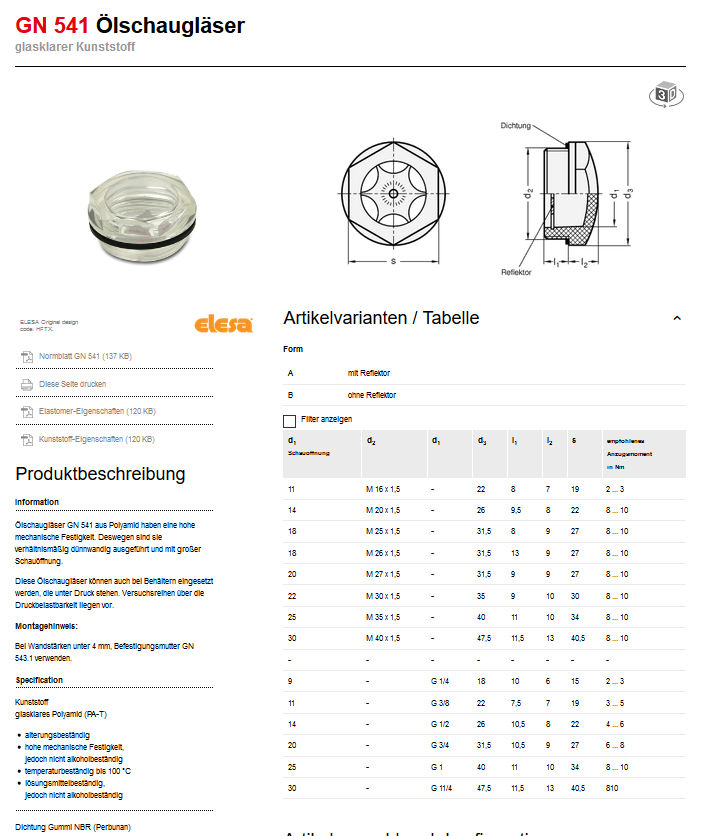
\includegraphics[width=1.1\textwidth,keepaspectratio]{figures/Oelschauglas.png}
	\caption{Datenblatt Ölschauglas \protect\cite{bib:www:schauglas}}
	%		\caption{Datenblatt Reibbelag\protect\ccite{bib:www:reibbelag}\protect\footnotemark}
	\label{fig:schauglas }
\end{figure}
\footnotetext{Vgl. [Gria] }

\newpage
\begin{figure}[H]
	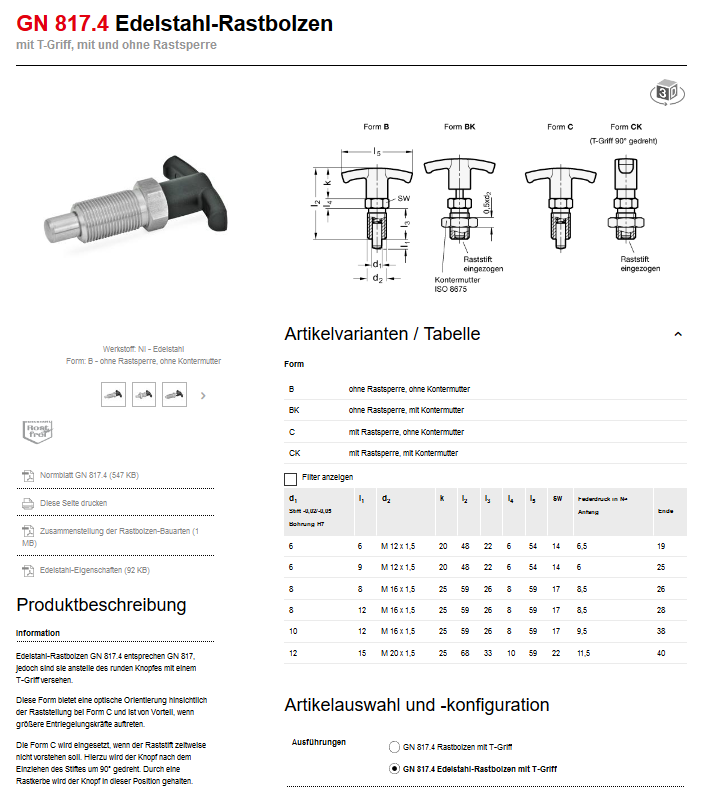
\includegraphics[width=1.1\textwidth,keepaspectratio]{figures/Rastbolzen.png}
	\caption{Datenblatt Arretierung Schaltung 1 \protect\cite{bib:www:rastbolzen}}
	%		\caption{Datenblatt Reibbelag\protect\ccite{bib:www:reibbelag}\protect\footnotemark}
	\label{fig:rastbolzen}
\end{figure}
\footnotetext{Vgl. [Grib] }

	\begin{figure}[H]
	\vspace{-2cm}
	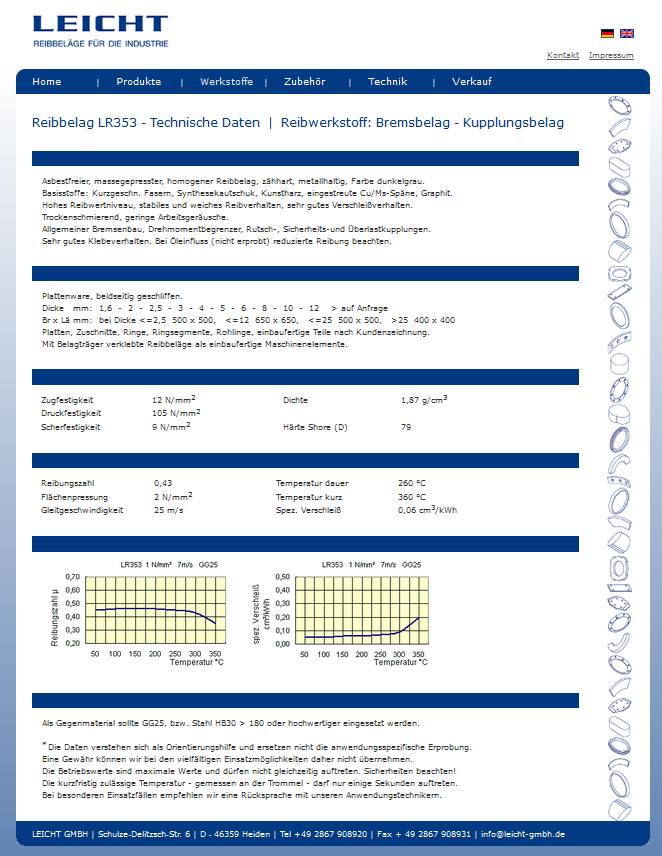
\includegraphics[width=1.0773\textwidth,keepaspectratio]{figures/Reibbelag.png}
	\caption{Datenblatt Reibbelag \protect\cite{bib:www:reibbelag}}
	%		\caption{Datenblatt Reibbelag\protect\ccite{bib:www:reibbelag}\protect\footnotemark}
	\label{fig:Reibbelag}
\end{figure}
\footnotetext{Vgl. [Gmb] }